\documentclass[10pt]{article}
\usepackage[margin=1in, paperwidth=8.5in, paperheight=11in]{geometry}
\usepackage{ifpdf,amsmath, amssymb, comment, color, graphicx, stmaryrd,setspace,enumitem,tikz, fancyhdr, wrapfig, textcomp, units, mathptmx, pdfpages, cancel, multicol}
\usepackage{hyperref}
\hypersetup{
    colorlinks=true,
    urlcolor=blue,
}

\setlength{\headheight}{14.5pt}
\newcommand{\Q}{\mathbb{Q}}
\newcommand{\R}{\mathbb{R}}
\newcommand{\Z}{\mathbb{Z}}
\newcommand{\vu}{\mathbf{u}}
\newcommand{\vv}{\mathbf{v}}
\newcommand{\vw}{\mathbf{w}}
\newcommand{\vi}{\mathbf{i}}
\newcommand{\vj}{\mathbf{j}}
\newcommand{\vk}{\mathbf{k}}
\newcommand{\vn}{\mathbf{n}}
\newcommand{\vr}{\mathbf{r}}
\newcommand{\va}{\mathbf{a}}
\newcommand{\vF}{\mathbf{F}}
\newcommand{\vL}{\mathbf{L}}
\newcommand{\vT}{\mathbf{T}}
\newcommand{\vN}{\mathbf{N}}
\newcommand{\proj}{\operatorname{proj}}
\newcommand{\orth}{\operatorname{orth}}
\newcommand\del\nabla
\newcommand\dotp[1][.5]{\,\mathbin{\vcenter{\hbox{\scalebox{#1}{$\bullet$}}}}\,}
\newcommand{\slice}{_\text{slice}}

% Solution text is in red. If you want the solutions to show, remove the \iffalse from the definition of the \red command.
%\newcommand{\red}[1]{ %\iffalse
%	\textcolor{red}{#1} }%\fi}

\newenvironment{red}{\color{red}}{\ignorespacesafterend}
\newenvironment{blue}{\color{blue}}{\ignorespacesafterend}
\newcommand{\green}[1]{\textcolor{green}{#1}}
\renewcommand{\section}[1]{\begin{center} \textbf{#1} \\\end{center}}
%
\hyphenpenalty=5000
\setlength{\parindent}{0in}
%\oddsidemargin=-.25in
\allowdisplaybreaks
\pagestyle{fancy}
\renewcommand{\headrulewidth}{0pt}
\lhead{MATH 202}
\rhead{Spring 2022}
%\lfoot{\copyright\ CLEAR Calculus 2010}
\cfoot{}

\begin{document}
%


%\onehalfspacing
\allowdisplaybreaks
%##################################################################
\section{PS\#6: Density, center of mass, and work - \red{Answer key} }

\everymath{\displaystyle}
\begin{enumerate}[leftmargin=0pt]

\item (\href{https://activecalculus.org/single/sec-6-3-mass.html#aQN}{APC 6.3 Exercise 6}) 
Consider two thin bars of constant cross-sectional area, each of length 10 cm, with respective mass density functions $\rho(x) = \frac1{1+x^2}$ and $p(x) = e^{-0.1x}$.
\begin{enumerate}
    \item Find the mass of each bar.
    
    \begin{red}
    The mass of bar $\rho$ is $\int_0^{10}\frac1{1+x^2}\, dx = \arctan(x)|_0^{10} = \arctan(10) - \arctan(0) = \arctan(10) - 0 \approx 1.4711.$
    
    The mass of bar $p$ is $\int_0^{10} e^{-0.1x}\, dx = \left.\frac{1}{-0.1} e^{-0.1x}\right|_0^{10} = (-10e^{-1}) - (-10e^{0}) = 10 - \frac{10}{e} \approx 6.3212.$
    \end{red}
    \item Find the center of mass of each bar.
    
    \begin{red}
    The center of mass of bar $\rho$ is
    \begin{align*}
        \frac{\int_0^{10}x\cdot \frac1{1+x^2}\, dx}{\int_0^{10}\frac1{1+x^2}\, dx} &=
        \frac{1}{\arctan(10)}\int_0^{10}\frac{x}{1+x^2}\, dx \quad (u = 1 + x^2; \ \ du = 2x\, dx) \\
        &= \frac{1}{\arctan(10)} \left[\frac12 \ln(1+x^2)\right|_0^{10}\\
        &= \frac{\ln(101)}{2\arctan(10)}
        \approx 1.5686
    \end{align*}
    
    The center of mass of bar $p$ is
    \begin{align*}
        \frac{\int_0^{10}x\cdot e^{-0.1x}\, dx}{\int_0^{10} e^{-0.1x}\, dx} &= \frac{1}{10-10/e}\int_0^{10} x e^{-0.1x}\, dx \quad \text{(integration by parts)} \\
        &= \frac{1}{10-10/e}\left[-10xe^{-0.1x} - 100e^{-0.1x}\right|_0^{10} \\
        &= \frac{1}{10-10/e}
            [(-10\cdot 10 \cdot e^{-1} - 
            100\cdot e^{-1})-
            (-10\cdot 0 \cdot e^0 - 100e^0)] \\
        &= \frac{1}{10-10/e}\left[\frac{-100}{e} - \frac{100}{e} + 0 + 100\right] 
        = \frac{100 - 200/e}{10 - 10/e} \approx 4.1802
    \end{align*}
    \end{red}
    \item Now consider a new 10 cm bar whose mass density function is $f(x) = \rho(x) + p(x)$.
    \begin{enumerate}
        \item Explain how you can easily find the mass of this new bar with little to no additional work.
        
        \begin{red}
        Since $\int_0^{10} (\rho(x) + p(x))\, dx = \int_0^{10} \rho(x)\ dx + \int_0^{10}p(x)\ dx$, the mass of the new bar is the sum of the masses of the earlier two bars. So, the mass of the new bar is $ \left(10 - \frac{10}{e}\right) + \arctan(10) \approx 7.7923.$
        \end{red}
        \item Similarly, compute $\int_0^{10} x f(x)\, dx$ as simply as possible, in light of earlier computations.
        
        \begin{red}
        Similarly, since $\int_0^{10} x(\rho(x) + p(x))\, dx = \int_0^{10} x\rho(x)\ dx + \int_0^{10} x p(x)\ dx$, this thing that would be in the numerator of the new center-of-mass calculation is the sum of the two previous numerators: \\
        $\tfrac{1}{2} \ln(101) + (100 - 200/e) \approx 28.7317.$
        \end{red}
        \item True or false: the center of mass of this new bar is the average of the centers of mass of the two earlier bars. Write at least one sentence to say why your conclusion makes sense.
        
        \begin{red}
        The new center of mass is $\frac{28.7317}{ 7.7923} \approx 3.6872;$ the average of the two earlier centers of mass is $\frac{1.5686 + 4.1802}{2} \approx 2.8744.$ It's a little surprising that these numbers are different, because it would make intuitive sense for the centers of mass to be related in this way. But, if you compare how the average of two fractions $a/b$ and $c/d$ would be computed to the fraction $\frac{a+c}{b+d}$ (which is called the ``mediant''), you'll see why it doesn't work out that way.
        
        (PS: This does work out to be the \textit{weighted} average of the centers of mass!)
        \end{red}
    \end{enumerate}
\end{enumerate}

\end{enumerate}
\end{document}

\item (\href{https://activecalculus.org/single/sec-6-4-physics.html#wrN}{AC 6.4 Exercise 7}) A cylindrical tank, buried on its side, has radius 3 feet and length 10 feet. It is filled completely with water whose weight density is 62.4 lbs/ft$^3$, and the top of the tank is two feet underground.
\begin{enumerate}
    \item Set up, but do not evaluate, an integral expression that represents the amount of work required to empty the top half of the water in the tank to a truck whose tank lies 4.5 feet above ground.
    
    \begin{red}
    First step: draw a picture and draw a slice. Your picture may of course be a little different -- perhaps in particular you may have chosen to draw a length down from the top of the tank to the slice, rather than the length I've drawn from the center up to the slice. I have both a picture of the overall tank situation and a picture of the end of the tank to help me figure out the relationship between the width of the slice and its height up from the center.
    
    \begin{center}
        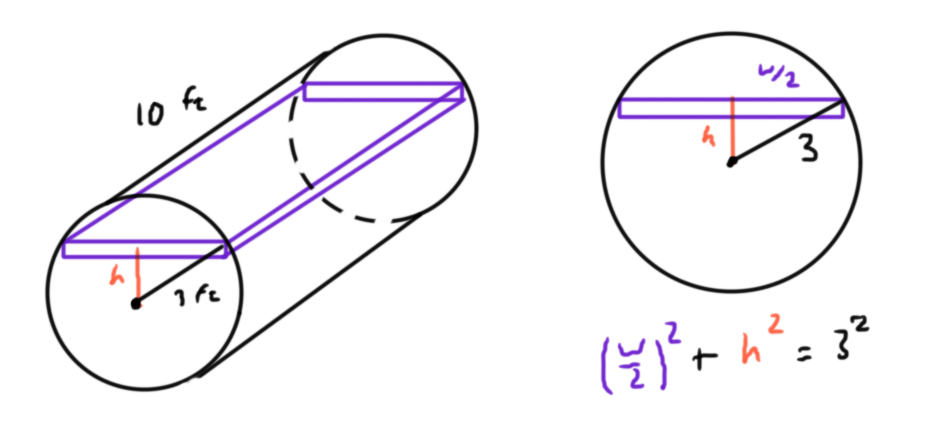
\includegraphics[width=0.7\textwidth]{images/fig-6.4.7.a.png}
    \end{center}
    Now we can figure out the work done to lift a slice. Notice that I'm using capital $W$ for ``work'' and lowercase $w$ for ``width'' -- this is moderately annoying but I believe in you. The work done to lift a slice is the force needed to lift the slice times the distance that slice will be lifted:
    \begin{align*}
        W\slice &= F\slice \cdot d\slice \\
        &= (V\slice\cdot\rho)\cdot d\slice \\ 
        &= (\ell\cdot w\slice \cdot \Delta h\cdot 62.4)\cdot d\slice \\
        \intertext{The width of the slice depends on $h$ in the way illustrated in the diagram. I've solved the equation I wrote for $w$:}
        &= (10\cdot 2\sqrt{9-h^2}\cdot \Delta h \cdot 62.4)\cdot d\slice \\
        \intertext{The slice at height $h$ needs to be lifted by $3-h$ to get to the top of the tank, then by 2 to get to ground level, then by 4.5 to get into the truck.}
        &= (10\cdot 2\sqrt{9-h^2}\cdot \Delta h \cdot 62.4)\cdot (3-h+2+4.5) \\
        &= (10\cdot 2\sqrt{9-h^2}\cdot \Delta h \cdot 62.4)\cdot (9.5-h) \\
        \text{Unit check:\quad \quad} 
        &= (\underbrace{10\cdot}_{\text{ft}}
        \underbrace{2\sqrt{9-h^2}}_{\text{ft}}\cdot 
        \underbrace{\Delta h}_{\text{ft}} \cdot 
        \underbrace{62.4}_{\text{lb / ft}^3})\cdot 
        \underbrace{(9.5-h)}_{\text{ft}} \quad \text{Yay, that's the right units.}
    \end{align*}
    Now we need to integrate from the center of the tank to the top of the tank. That's from $h=0$ to $h=3$. Therefore, the integral computing the amount of work is
    \[W_\text{total} = \int_{h=0}^3 (10\cdot 2\sqrt{9-h^2} \cdot 62.4)\cdot (9.5-h)\ dh.  \]
    \end{red}
\end{enumerate}